\documentclass[12pt]{article}

\usepackage[portuguese, english]{babel}
\usepackage[T1]{fontenc}
\usepackage[a4paper, left=3cm, right=2cm, top=3cm, bottom=2cm]{geometry}
\usepackage{authblk}
\usepackage{cite}
\usepackage{fontspec}
\usepackage[toc]{glossaries}
\usepackage{graphicx}
\usepackage{hyperref}
\usepackage{setspace}
\usepackage{subcaption}
\usepackage{verbatimbox}
\usepackage[dvipsnames]{xcolor}

\addto\captionsportuguese{\renewcommand*\contentsname{Sumário}}

\newcommand\myshade{85}
\newcommand{\pprime}{\ensuremath{^{\prime}}}
\newcommand{\RNum}[1]{\uppercase\expandafter{\romannumeral #1\relax}}

\hypersetup{
    pdftitle   = {Consequências da dependência tecnológica do indivíduo moderno - Um ensaio analítico e reflexão sobre perspectivas futuras},
    pdfauthor  = {Autor Anônimo},
    pdfsubject = {Este artigo tem como propósito explorar as consequências associadas à crescente dependência tecnológica
    do indivíduo moderno na sociedade contemporânea.},
    linkcolor  = black,
    citecolor  = black,
    urlcolor   = black,
    colorlinks = true,
    filecolor  = black,
    linktoc    = page
}%

\newglossaryentry{ict} {
  name={ICT},
  description={
    Tecnologia da Informação e Comunicação (\textbf{ICT}, do inglês: \textit{Information and Communications Technology},
    ou \textbf{TIC}, em português) é um termo extensional para tecnologia da informação (\textbf{TI}) que enfatiza o papel das comunicações
    unificadas e a integração de telecomunicações (linhas telefônicas e sinais sem fio) e computadores, bem como software
    empresarial necessário, middleware, armazenamento e audiovisual, que permitem aos usuários acessar, armazenar, transmitir,
    entender e manipular informações \cite{techTarget2023}.
  }
}

\newglossaryentry{dependencia} {
  name={Dependência Tecnológica},
  description={
    O termo ``\textbf{dependência tecnológica}'', como empregado neste artigo, refere-se principalmente à relação de um
    indivíduo ou comunidade com algum recurso tecnológico ou provedor deste recurso, de modo que a relação desenvolvida
    caracterize uma espécie de natureza assimétrica \cite[1]{secretariat1977}, ou seja, na qual o indivíduo (ou
    comunidade) depende do recurso e/ou provedor de forma unilateral. Relações desta espécie frequentemente estão
    ligadas ao uso de tecnologias que dependem, de alguma forma, da relação com alguma organização de larga escala
    (\textit{organization-dependent technology} \cite[\S207-212]{kaczynski1995}) que possibilita a adoção desta
    tecnologia; desta maneira, o indivíduo (ou pequena comunidade) está a mercê da organização de larga escala à partir
    do momento que depende desta tecnologia para algum fim.
  }
}

\title{%
  Consequências da dependência tecnológica do indivíduo moderno\\
  \large Um ensaio analítico e reflexão sobre perspectivas futuras
}
\author[1]{Autor Anônimo}
\date{\today}
\affil[1]{Departamento de Informática e Estatística, Universidade Federal de Santa Catarina}

\makeglossaries

\begin{document}
\selectlanguage{portuguese} 
\begin{titlepage}
\maketitle
\thispagestyle{empty}

\begin{abstract}
  Este artigo tem como propósito explorar as consequências associadas à crescente dependência tecnológica do indivíduo
  moderno na sociedade contemporânea e como estas consequências se equiparam aos desenvolvimentos oriundos da
  modernização da civilização humana desde a primeira revolução industrial, dando atenção especial à forma que a aceleração 
  do avanço tecnológico pode agravar a marginalização e isolamento social de grupos digitalmente desfavorecidos e desencorajar a 
  autonomia do indivíduo e sua escolha em ativamente exercer suas funções na sociedade de forma saudável.
\end{abstract}

\end{titlepage}

\tableofcontents

\printglossary[title=Glossário, toctitle=Glossário]

\newpage

\section{Introdução}

Entre os anos de 2016 e 2022, a parcela da população brasileira que utiliza a Internet no cotidiano cresceu de 66,1\%
para 87,2\% \cite{carmennery2024}. O crescimento na adoção de \gls{ict}s observado na realidade do nosso país não é um
fenômeno isolado, e sim um reflexo do ritmo acelerado de modernização e digitalização da civilização contemporânea em escala
global \cite{jeffburt2010}. 

Por conseguinte, discussões sobre as possíveis consequências sociais, sistêmicas e
individuais do progresso tecnológico desabalado são um tópico comum nos campos de estudo da economia, sociologia,
geopolítica e estudos ambientais desde meados do século \RNum{20} \cite{kaczynski1995,marcusekellner2001}. Este artigo toma como base a
extensa literatura desenvolvida sobre estes tópicos no último século para articular um processo de análise e reflexão
em relação o impacto da modernização da sociedade como sistema sobre o indivíduo, nos aspectos de vida cotidiana, bem
estar físico e psicológico, autonomia, liberdade e socialização.

\section{Desenvolvimento}

\subsection{Desenvolvimento tecnológico como um indicador de problemas sociais}\label{indicador}

O primeiro ponto a ser evidenciado há de ser o alicerce do argumento principal da discussão proposta: existe, de fato,
uma correlação observável entre o grau de adoção tecnológica no contexto da existência de uma comunidade e a incidência de
problemas sociais --- sejam estes individuais ou sistêmicos? A verdade é que, para este tipo de questionamento, as
respostas encontradas dificilmente são achados concretos; é possível, no entanto, inferir à partir estudos estatísticos, se
há, ou não há, base para discussão acadêmica sobre dado postulado. No caso em questão, como pode-se intuir puramente à partir
da quantidade de estudos e ensaios publicados tratando do tema nas últimas décadas
\cite{secretariat1977,marien1977415}, sugerir que o progresso tecnológico da sociedade pode
ser um fator que mantém uma correlação com tendências problemáticas no desenvolvimento e vivência dos indivíduos que a compõe
não é algo de novo e, segundo as estatísticas indicam, não é nenhum equívoco: estudos conduzidos nos últimos cinco anos
identificam que muitas características da vida moderna --- produtos da revolução industrial \textit{especialmente} acentuados na
vivência urbana --- como disparidades sociais, poluição ambiental ou escassez de \textit{greenspace} podem ser
identificados como fatores contribuintes para os níveis elevados de incidência de problemas de saúde mental observados
em populações urbanas em países desenvolvidos \cite[1]{XU2023299}.

\begin{figure}[h]
    \centering
    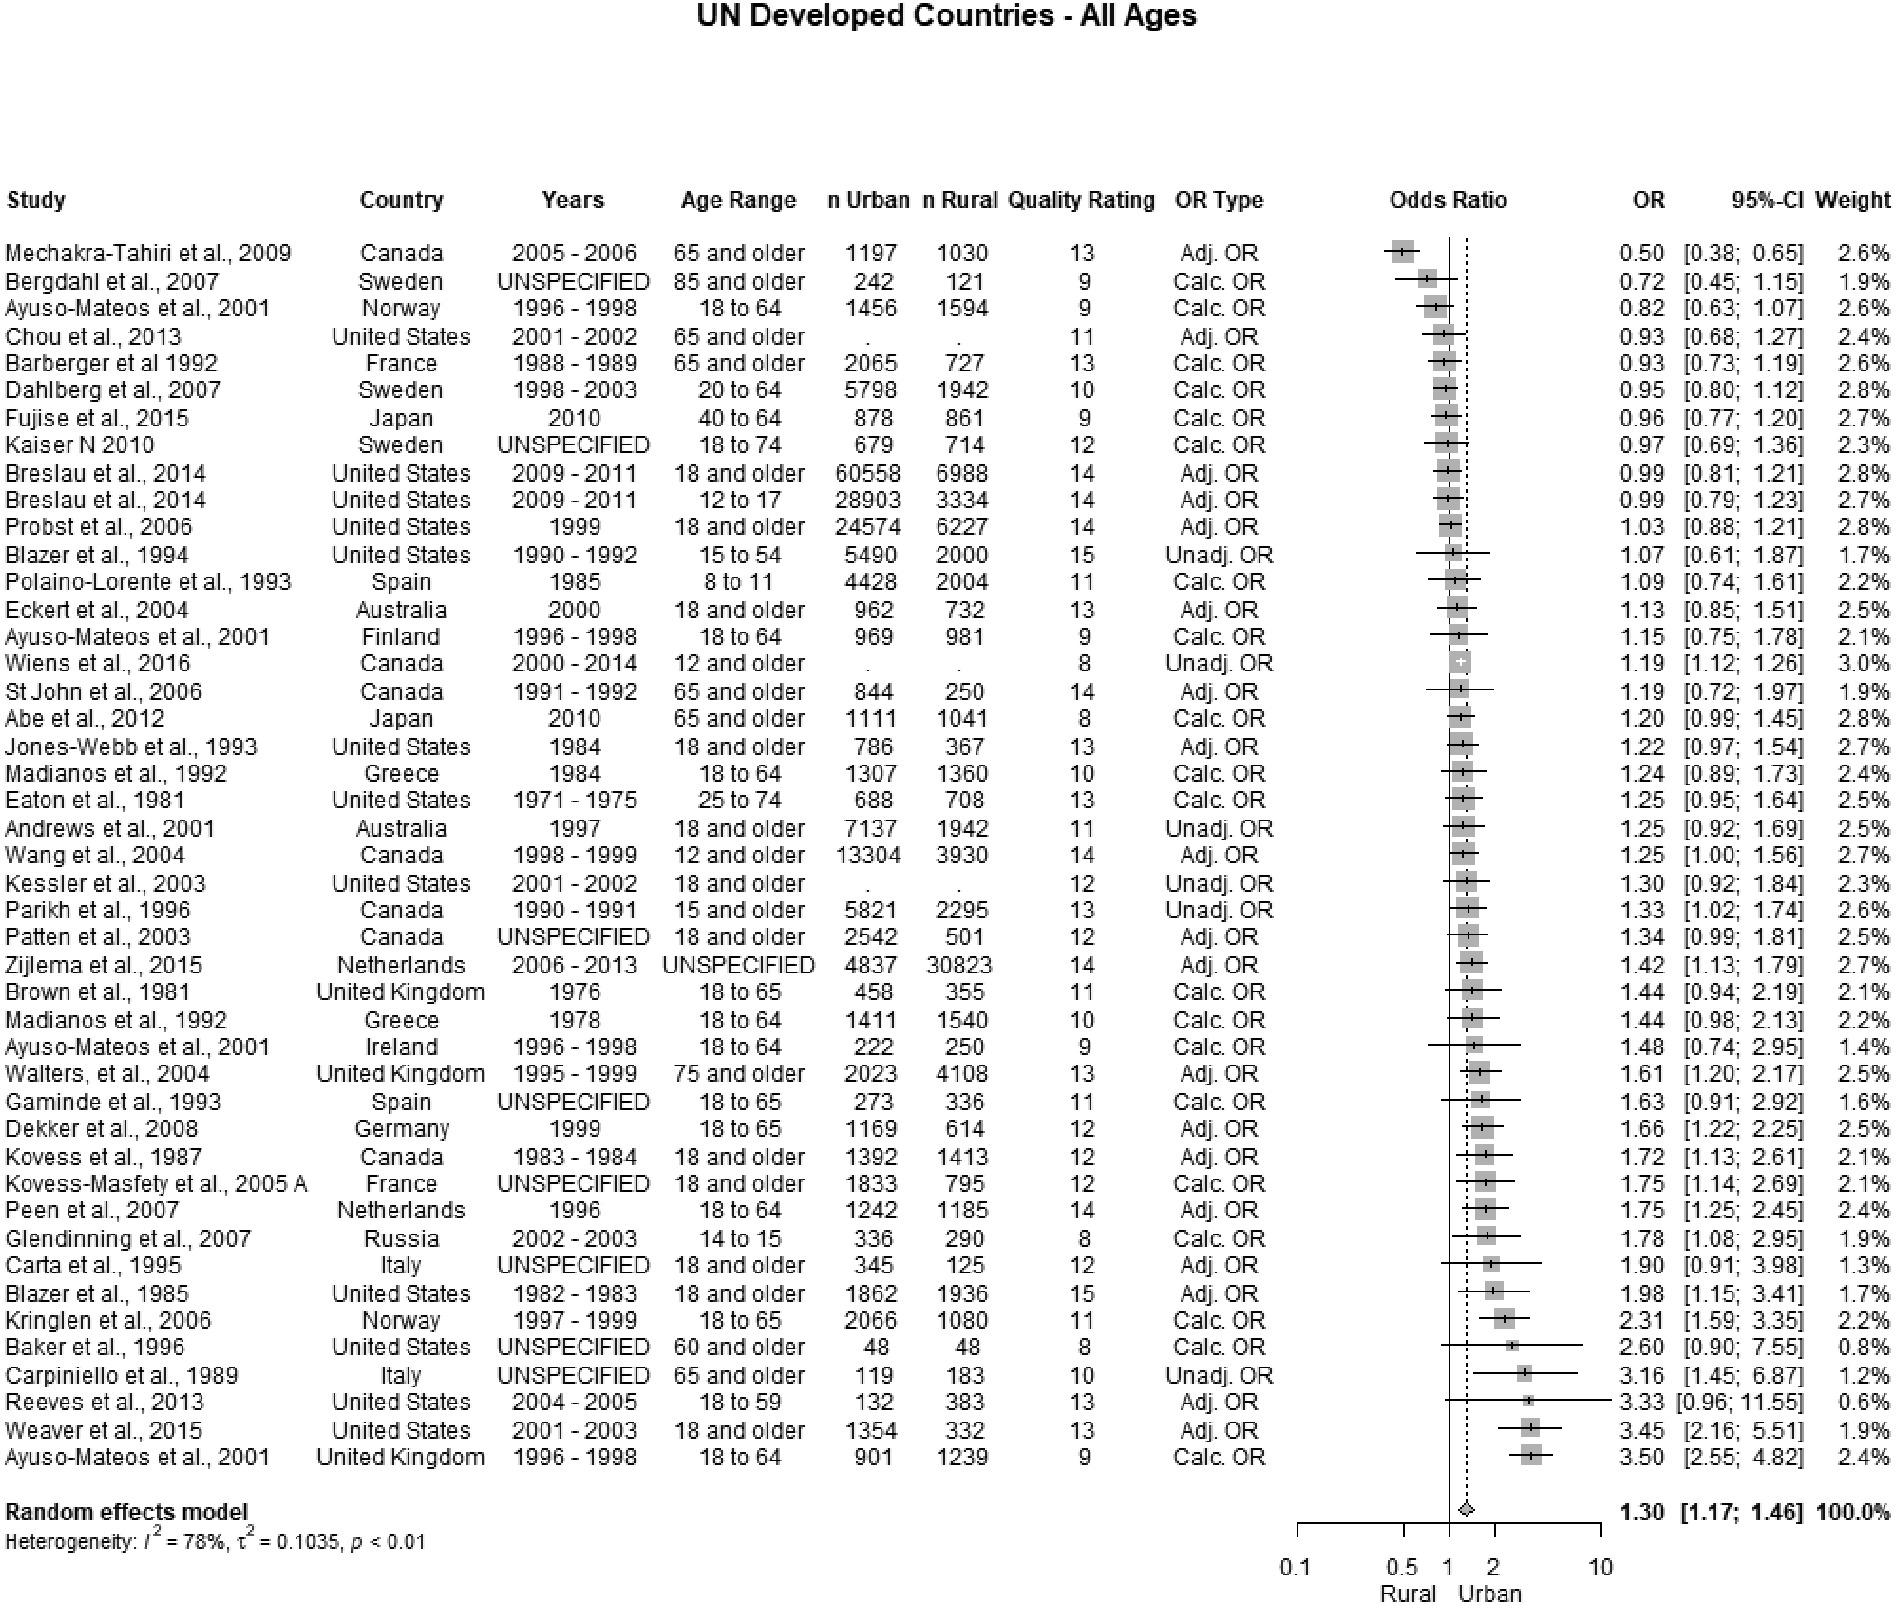
\includegraphics[width=15cm]{Content/Images/depression_rate.jpg}
    \caption{Incidência de depressão entre populações urbanas vs.\ rurais em países industrialmente desenvolvidos. Modelo
  matemático. \cite{XU2023299}}
\end{figure}

Como pode ser encontrado em estudos de até quatro décadas atrás, o grau de adoção e \gls{dependencia} de uma comunidade tem
um efeito não somente sobre a dinâmica econômica e social da realidade dos indivíduos nesta inseridos, mas pode mesmo
influenciar o condicionamento psicológico e valores característicos na paisagem cultural comunal \cite[27-30]{secretariat1977}.
Desta forma, fica evidente que os impactos da \gls{dependencia} devem ser estudados não apenas na escala \textit{macro},
mas que uma análise de escopo individual também é necessária.

\subsection{Autonomia e senso de liberdade}\label{autonomia}

A complicação atrelada de forma mais aguda a um crescente nível de \gls{dependencia} é, por definição, a perda de autonomia do
sujeito, seja ele individual ou coletivo, perante ao fim para qual a tecnologia adotada é um meio (se qualquer; como
será explorado adiante, um fator oriundo do processo pelo qual a dependência se forma é o surgimento de necessidades
artificiais à serem supridas \cite[\S59-65]{kaczynski1995}; ver parágrafo \ref{necessidades_artificiais}) e o surgimento
da relação de dependência assimétrica onde este sujeito torna-se subjugado ao provedor da tecnologia organizacional
\cite[27-30]{secretariat1977}.

A ocorrência desta espécie de relação desequilibrada segue um padrão conhecido: o processo de submissão
econômica e tecnológica é, em determinado aspecto, um processo histórico. Análise macroscópica de relações
internacionais envolvendo troca de \textit{commodities} entre nações em desenvolvimento e potências industriais reflete
este padrão de assimetria nos tipos de bens capitais trocados por cada parte, que se manifesta na escala individual
através da (escassez de) diversidade de oportunidades econômicas disponíveis para indivíduos e comunidades que compõem
sociedades tecnologicamente subdesenvolvidas como consequência da desvantagem sistêmica manifestada pela diferença no
grau de desenvolvimento tecnológico e, assim, nos meios de produção \cite[27-30]{secretariat1977}. Desta forma, ao
analisarmos esta situação sob o escopo da experiência individual, observamos a emergência de um outro padrão cujo o
estudo é instrumental para a compreensão dos impactos sociais causados pela aceleração tecnológica: a limitação da gama
de possibilidades que compõe a realidade do indivíduo como consequência da busca pelo avanço tecnológico absoluto
\cite[\S51]{kaczynski1995}.

Este padrão ocorre não apenas na variedade de atividades econômicas acessíveis para dada parcela da população, mas de
forma universal ao passo que o progresso tecnológico em si passa a significar a aceleração do próprio sistema e não mais
a priorização do avanço e melhoria da situação humana. Observa-se que o progresso tecnológico que, em um primeiro
momento, tem o propósito de possibilitar a expansão do potencial humano, logo torna-se o objeto do esforço que restringe
as liberdades do indivíduo \cite[\S127]{kaczynski1995}; como um exemplo prático, pode ser empregada uma análise do caso
do transporte motorizado, que no momento de sua invenção, apresentava uma solução para o transporte rápido entre pontos
excepcionalmente distantes --- um século após a popularização do automóvel, este tornou-se essencialmente indispensável
para a vivência moderna, como as cidades e os espaços de vivência passaram a ser projetados para os carros, não para os
homens. Desta forma, a sociedade adequa-se para acomodar o avanço tecnológico e é moldada por ele; para
o indivíduo, o progresso inabalado da tecnologia é algo que é imposto sobre ele, sobre o qual não tem autonomia e deve,
assim como a sociedade em que está inserido, adequar-se. Quando a tecnologia em questão é de ordem organizacional (ver
glossário \cite[\S207-212]{kaczynski1995}) existe um efeito composto caracterizado por não somente a dependência sobre o
recurso em si, mas também sobre a relação com o elemento que provê esta tecnologia, que então exerce uma relação de
dominância sobre o usuário subjugado, neste caso, o indivíduo.

Com o surgimento e normalização desta dinâmica na vivência urbana contemporânea, é possível que um dos fatores
causadores da elevada incidência de casos de depressão e outros transtornos psicológicos reportados pelas populações
urbanas esteja ligado ao senso de submissão ou à percepção de uma falta de autonomia perante o sistema --- como indicam
estudos fundamentais sobre a psique humana, a maioria das pessoas percebe uma inata necessidade de liberdade e autonomia
para o processo de auto-realização \cite{nietzsche2011will}, o que \textbf{não significa} que a tecnologia, como um
fato, seja um empecilho para o desenvolvimento individual, ou mesmo a dependência sobre esta; o que sugerimos, assim
como muitos estudos anteriormente \cite{kaczynski1995, secretariat1977}, é que a \textbf{imposição da dependência 
tecnológica sobre o indivíduo, de forma sistêmica e constante}, é um fator agravante para os problemas observados.

\subsubsection{Autonomia e independência na era digital}

A chegada da era digital e o surgimento e universalização das mídias social (ou redes sociais) como fato social
representa não apenas um agravante à situação de dependência descrita --- centralizando os meios de comunicação e
propagação de informação nas mãos de um pequeno número de \textit{megacorporações}, causando assim a dependência sobre
estes agentes provedores --- como também a origem de um outro fator que mantém uma correlação observável ao aumento no
índice de transtornos psicológicos na sociedade moderna: o senso de isolamento e inadequação na presença da grande quantidade
de relações ``rasas'' mantidas apenas através dos meios virtuais: segundo estudos conduzidos na última década pela
\textit{Santa Clara University}, uso excessivo de mídias sociais está atrelado à um índice elevado de comportamento
anti-social e auto destrutivo \cite[1]{amediejacob2015}.

\subsection{Percepção de inadequação}

Temas relacionados à auto-estima e auto-percepção são bastante comuns no discurso tratando dos impactos da popularização
de mídias sociais. As mídias sociais possibilitaram o acesso à uma plataforma onde qualquer pessoa pode, à sua
vaidade, representar os eventos da própria vida na luz que mais a favorece \cite{affiziedoes}.
Como descrito pelo psicólogo americano Leon Festinger, o impulso humano de auto-comparação
\cite{festinger1957social} manifesta-se muitas vezes de forma destrutiva quando em contato com o imagético cultural
produzido por estas plataformas. Os efeitos deste excesso de exposição às redes está, também, associado aos sentimentos
de isolamento e inadequação descritos anteriormente \cite[1]{amediejacob2015}, e quem sabe isso seja por
\textit{design}.

O crescimento da dependência tecnológica tem revelado um impacto significativo na saúde mental das populações modernas.
Estudos recentes indicam que o uso prolongado de dispositivos digitais e redes sociais está correlacionado com níveis mais
elevados de ansiedade e depressão, especialmente entre jovens adultos e adolescentes \cite[amediejacob2015]. A constante 
exposição a um fluxo de informações cuidadosamente curadas nas mídias sociais pode levar a uma percepção distorcida da realidade,
onde o indivíduo se sente pressionado a atingir padrões irreais de sucesso, beleza e felicidade. Esse fenômeno
intensifica o sentimento de inadequação, gerando um ciclo de comparação social negativa e baixa autoestima.
Além disso, a dependência das validações instantâneas — como curtidas e comentários — pode agravar sentimentos de solidão
e isolamento, criando um paradoxo onde a busca por conexão digital resulta em um maior distanciamento das interações sociais reais.

Um outro efeito colateral importante da dependência tecnológica é o impacto no discurso público e na polarização social. 
A personalização de conteúdos promovida pelos algoritmos das plataformas digitais cria bolhas informativas que reforçam
as crenças pré-existentes dos usuários, limitando a exposição a perspectivas contrárias \cite{okeefe2011}. Esse
fenômeno, conhecido como "efeito de câmara de eco", pode levar ao aumento da polarização política e à radicalização d
e opiniões, enfraquecendo o debate saudável e plural que é fundamental para uma democracia robusta. Além disso, a disseminação
de fake news e desinformação através dessas plataformas pode influenciar significativamente a opinião pública,
afetando processos eleitorais e decisões políticas, como foi amplamente documentado em casos recentes ao redor do mundo.

\subsubsection{Necessidades artificiais}\label{necessidades_artificiais}

As mídias sociais representam também uma nova e mais efetiva plataforma de propaganda (para os propósitos deste
argumento, o termo ``propaganda'' refere-se estritamente ao sentido \textit{comercial} da palavra, apesar de que a
distinção entre propaganda comercial e política nem sempre é tão simplesmente traçada) do que os modelos observados
anteriormente na sociedade: a possibilidade de exposição à publicidade à qualquer hora do dia por períodos extensos de
tempo, como viabilizado pela popularização dos \textit{smartphones} e mídias sociais significam uma acentuação dos
efeitos observados com outros tipos de propaganda previamente, como a televisão, ou em programas de rádio
\cite{okeefe2011}. Este fenômeno está associado à um aumento no comportamento compulsoriamente consumista, sim, mas
também, de forma mais sutil, está relacionado ao condicionamento psicológico que determina a percepção do que é
``normal'' e, como queremos destacar, do que é ``necessário'' \cite[3]{jameshulbert1968}.

O processo pelo qual as práticas de publicidade e propaganda criam a percepção de necessidades que não existiam anteriormente
é estudado desde, pelo menos, meados do século \RNum{20} \cite[3]{jameshulbert1968}. A criação desta percepção
é um exemplo concreto de como o ambiente produzido pelo avanço tecnológico
pode ser usado como uma forma de condicionamento psicológico poderosa, assim como uma demonstração prática da criação
artificial de adversidades sobre o indivíduo. Os efeitos observados nos
resultados dessa análise são indiscutivelmente exacerbados pelo advento da universalização destas ferramentas de
publicidade através das mídias sociais modernas. Argumentamos que o senso desta nova gama de necessidades não supridas
está, possivelmente, associado aos elevados níveis de transtornos psicológicos identificados em análises estatísticas
atuais, em conjunto com os outros fatores mencionados neste texto.

\section{Reflexão}

Após análise dos pontos levantados, a seção de ``Reflexão'' tem o propósito de fornecer algumas conclusões e
\textit{insights} sobre o mundo onde vivemos e como melhor nos relacionarmos com este no cotidiano.

\subsection{Cenário atual}

Como explorado na seção de Desenvolvimento (\ref{indicador}, \ref{autonomia}), vivemos em um mundo onde um certo grau de
dependência tecnológica é, para a maioria, inevitável. A tendência global indica que as populações urbanas estão em
crescimento, e que por volta do ano 2050, dois terços de toda a população mundia residirá em áreas urbanas
\cite{nations2014world}. Por isso é importante ter consciência sobre os impactos que as relações formadas pelo avanço da
tecnológica têm sobre o indivíduo, especialmente para aqueles que tem dificuldades em levar uma vida saudável e/ou
sofrem de transtornos psicológicos ou por consequência de problemas sociais.

\subsection{Consumo consciente}

No contexto atual, a alfabetização digital torna-se uma competência fundamental para a cidadania plena. Não se trata apena
s de habilidades técnicas, como o uso de ferramentas e plataformas, mas também de competências críticas para analisar informações,
identificar fake news e compreender os impactos éticos das tecnologias. Para que a sociedade possa navegar de forma consciente
em um ambiente digital saturado, é essencial investir na educação digital desde os primeiros anos escolares. Isso inclui
o desenvolvimento do pensamento crítico, a capacidade de distinguir entre fontes confiáveis e tendenciosas, e a promoção
de comportamentos responsáveis nas redes sociais. Ao capacitar os cidadãos para interagir de forma crítica e ética com
as tecnologias, é possível reduzir a vulnerabilidade a manipulações e promover um uso mais sustentável e responsável das
plataformas digitais.

À medida que o volume de informações disponíveis online cresce exponencialmente, o consumo consciente de conteúdo torna-se
uma habilidade essencial para a saúde mental e o bem-estar digital. A prática envolve selecionar cuidadosamente as fontes
de informação, priorizando qualidade sobre quantidade, e evitando o consumo excessivo que pode levar à sobrecarga cognitiva
e ansiedade. Além disso, é fundamental questionar a veracidade das informações, exercitando o pensamento crítico para
identificar fake news, manipulações e vieses ocultos. Adotar um consumo consciente não significa apenas proteger-se contra
desinformação, mas também cultivar um uso mais saudável e intencional da tecnologia, promovendo um equilíbrio entre a vida
online e offline. Isso inclui estabelecer limites para o tempo de tela, silenciar notificações que causam distrações constantes
e escolher plataformas que favoreçam interações positivas e construtivas. Dessa forma, o consumo consciente de conteúdo
pode ajudar a reduzir o estresse digital e contribuir para um uso mais sustentável e significativo das tecnologias modernas.


\newpage
\section{Referências Bibliográficas}
\bibliographystyle{apalike}
\bibliography{references}

\end{document}

